\newpage

\section*{ Indium  (Cd) }

Power Level: 1.0 kW(th) \\
Time at Power: 60 s \\
Wait Time: 400 s \\
Total Activity at Removal: 8.85e+01 $\mu Ci$

\begin{table*}[h]
\centering
\begin{tabular}{ |c|c|c|c|c|c|c| }
 \hline
 Position & Mass $mg$ & Start Counting $s$ & Counting Time $s$ & Counting Activity $\mu Ci$ \\
 \hline 
 1 & 1.7 & 460 & 300 & 2.23e+01\\ 
\hline
 2 & 1.5 & 760 & 300 & 1.84e+01\\ 
\hline
 3 & 1.4 & 1060 & 300 & 1.61e+01\\ 
\hline
 4 & 1.6 & 1360 & 300 & 1.73e+01\\ 
\hline
\end{tabular}
\end{table*}

\begin{figure}[!ht]
   \centering
   \subfloat[][Position \#1]{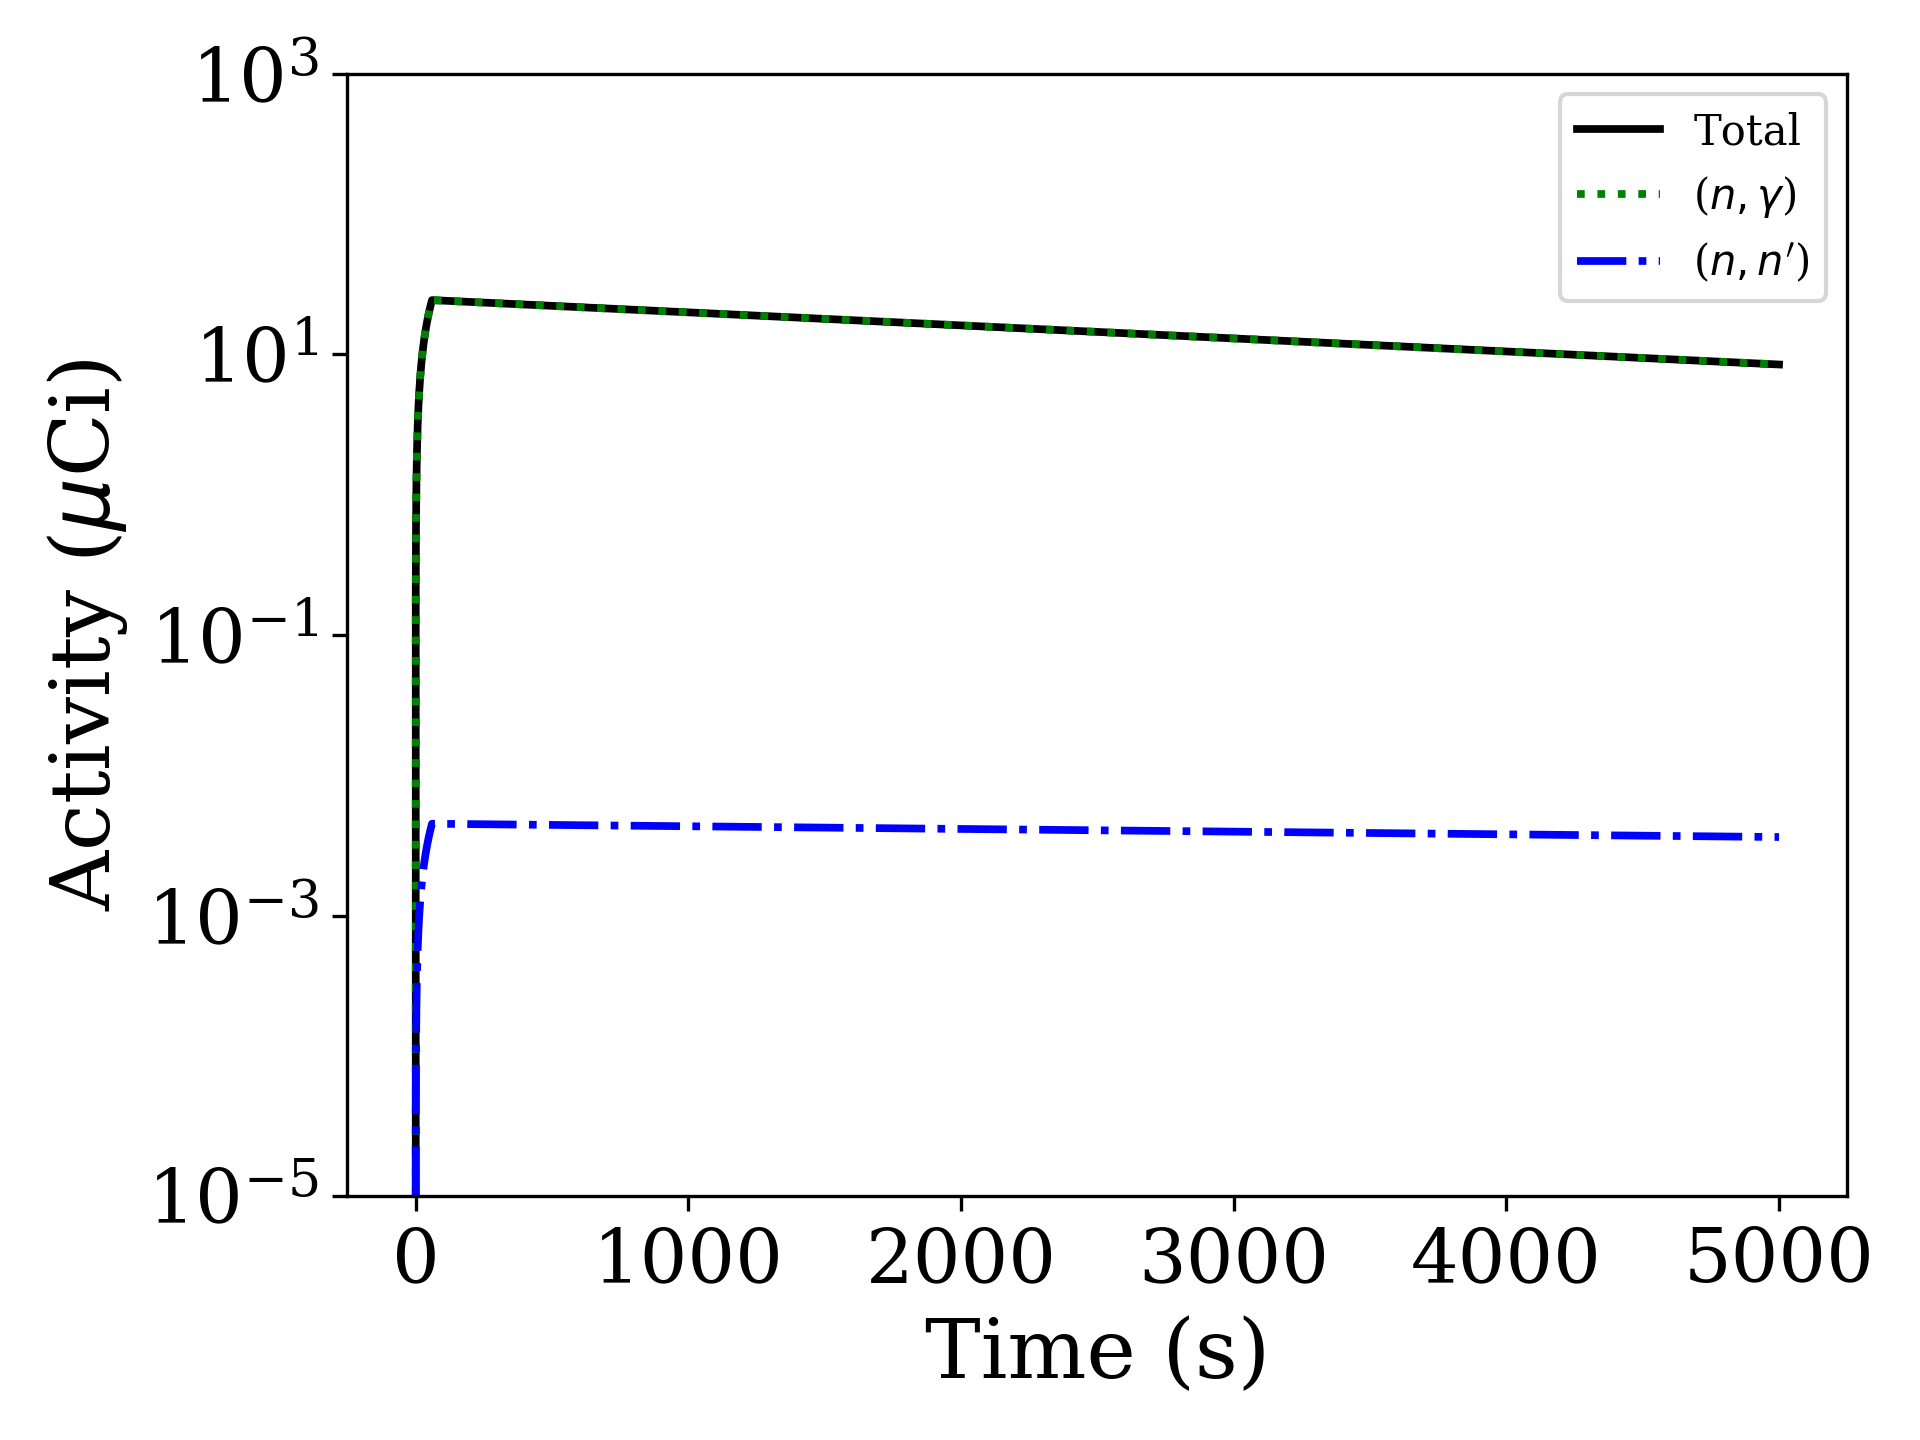
\includegraphics[width=.4\textwidth]{source/plot/in1cd_activity}}\quad
   \subfloat[][ ($n,\gamma$) Reaction Rate]{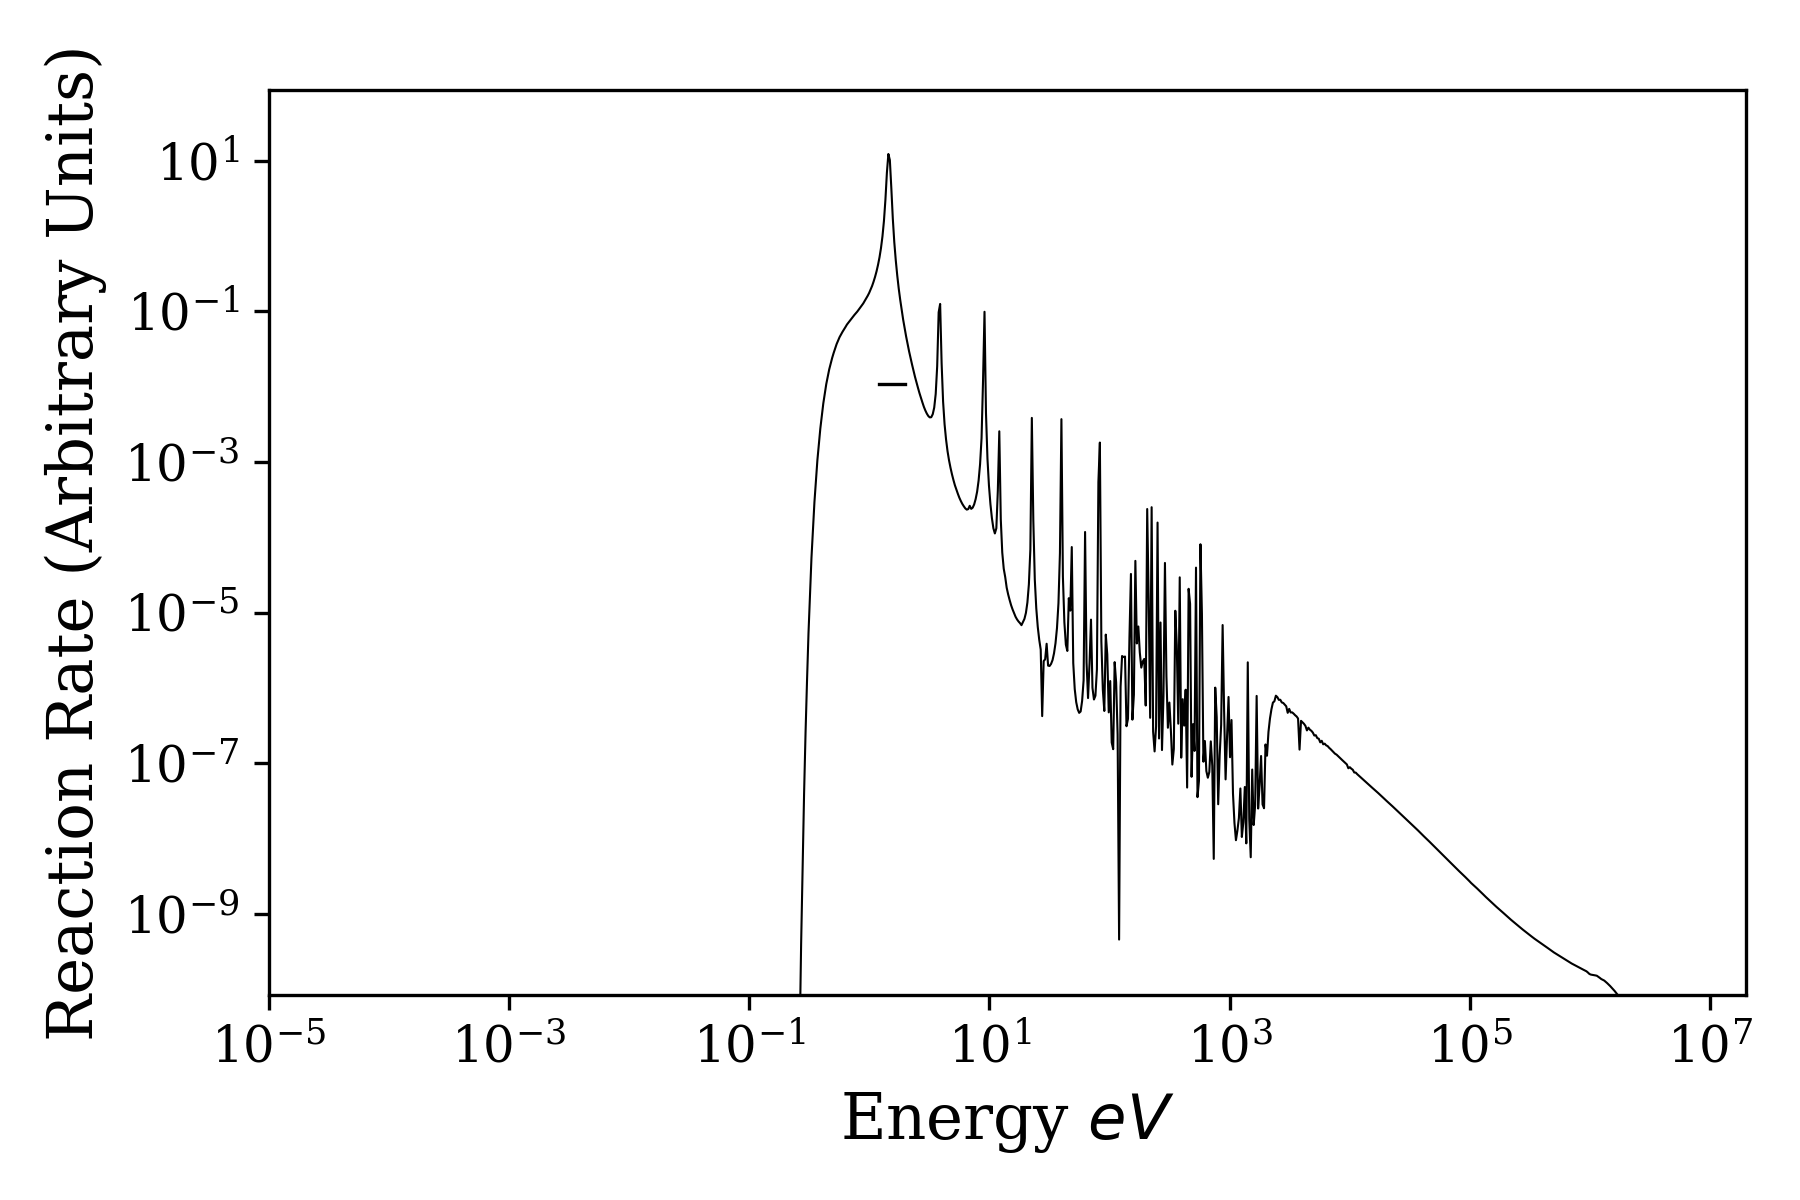
\includegraphics[width=.4\textwidth]{source/plot/in_n,gamma_cd}}\\ 
   \subfloat[][ ($n,n'$) Reaction Rate]{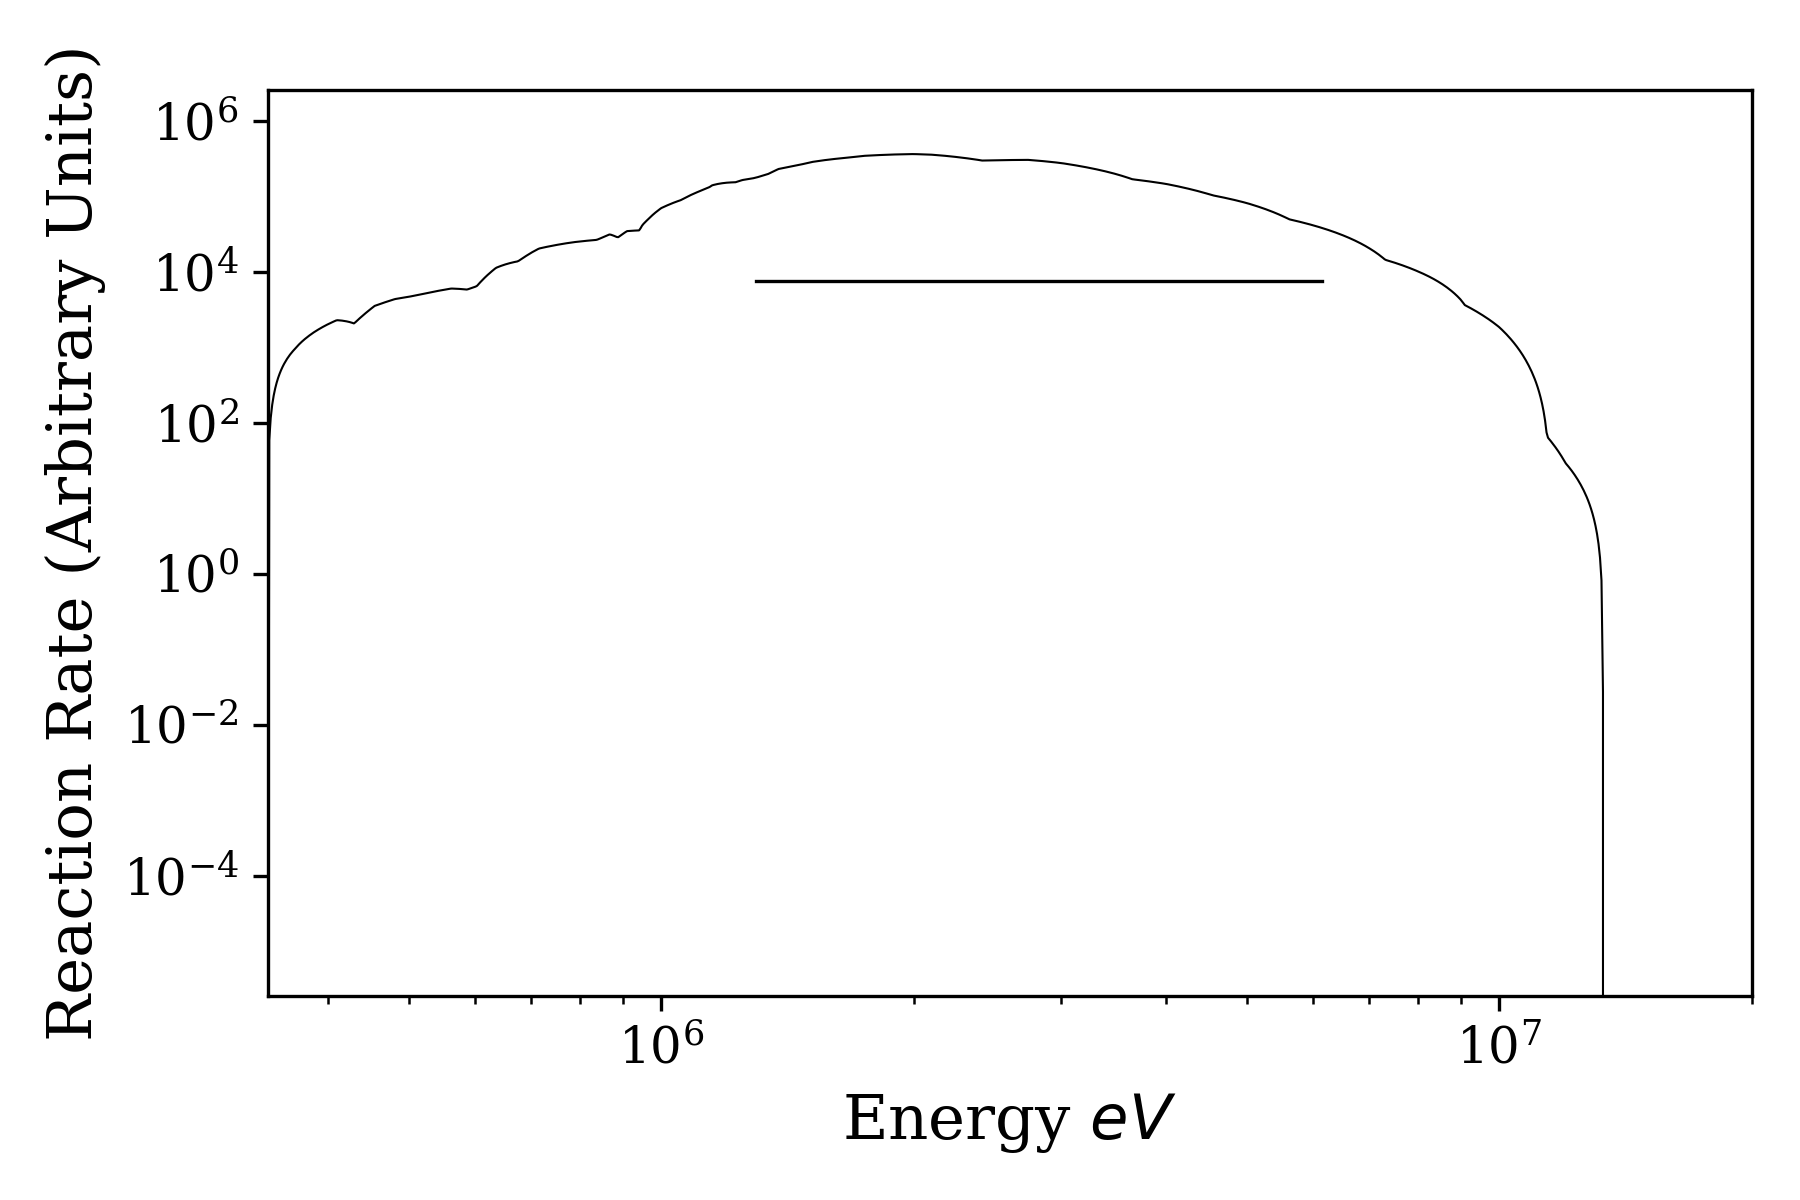
\includegraphics[width=.4\textwidth]{source/plot/in_n,inelastic_cd}}\quad 

\end{figure}

\begin{table*}[h]
\centering
\begin{tabular}{ |c|c|c|c|c|c|c| }
 \hline
 Reaction & T$_{1/2}$ & ROI (eV) & Important Gammas (keV) \\
 \hline 
 ($n,\gamma$) & 54.0 m & 1.20e+00, 1.99e+00 & 138(0.03), 417(0.36), 819(0.17), 1090(0.53), 1293(0.8), 1508(0.11), 2111(0.2) \\ 
\hline
 ($n,n'$) &  4.4 h & 1.34e+06, 5.97e+06 & 335(0.5) \\ 
\hline
\end{tabular}
\end{table*}
